\chapter{Adaptive Compression}

\label{ch:adaptivecompression}

\section{Cracking}

In this chapter we examine ways of performing online compression of the adjacency list representing
the graph by modifying the existing cracking algorithms presented by Ideos' et al.. The background
subsection on cracking covers the terms we will use in this chapter to explain the modifications we
made.

Our motivation for applying compression to cracking is to be able to run algorithms faster by exploiting uniform sections of the cracker column.

In this chapter, we will first discuss how we recognize opportunities to compress contiguous, uniform values within the cracker column. Then we will discuss the ways in which the information required to repeatedly exploit these uniform sections of the column can be stored. In the relevant sections and subsections we will describe our implementation of various techniques, which we see the evaluation of the next chapter.

\section{Opportunities}

Given an adjacency list which we are querying using cracking, we can gather information about uniform column-sections with varying eagerness in the course of a cracking scan. We can reserve a decision on compression until we know that an entire column-fragment is compressible, or we can make many small compressions while scanning a fragment of the cracker column.

When we compress only after identifying an entirely uniform column fragment, we call this "per-fragment" compression, because we are compressing entire column-fragments only.

Applying compression during the course of a scan is "eager" compression. Within the space of possibilities for eager compression, we have only explored run-length encoding (RLE) in this project.

\subsection{Per-fragment}

\label{ss:perfrag}

When applying per-fragment compression, we update the cracker index with the boundary values for any created fragment(s) after performing the column scan. If two stored indices are \textit{minimally different}, then we can compress the column in that range, which corresponds to a uniform column-fragment. Minimal difference between stored values is important to per-fragment compression for this reason, and later in this subsection we will explain the concept in more detail.

Advantageously, this method is very easy to implement. One must simply check the boundaries of newly created fragments and determine if any fragments can now be known to be uniform. The cost of this technique on top of normal cracking is a branch in which the cracker index is checked to see if the column fragment under consideration is uniform, meaning the selection can return early.

\subsubsection{Minimal Difference}

We use the phrase \textit{minimally different} to describe two values for which there exists no value between them in the range of values that can be taken for their common type. For example, if we consider the integers, the values 2 and 3 are minimally different, because there exists no integer between these values. For a data-type such as a floating point number, this value will vary depending on the accuracy with which the user wishes to cluster - it may be acceptable to the application that the values 2.33334 and 2.33279 both be considered 2.33, however, unlike in the integer case, there is information being lost during compression, which may not be acceptable to the user. In this case they may opt to use an appropriately fine granularity for the compression according to their application.

\subsection{Run-length Encoding}

Our aim with run length encoded cracking is to be able to speed up the scan by enabling scanning pointers to hop over long runs of the same value. For this, we build and maintain information about all runs of consecutive nodes in the cracker column. This is done inside an array called $run\_lengths$. $run\_lengths[i]$ indicates to a scanning pointer that the next \texttt{i} values (inclusive) are the same, and therefore can be considered together, whether that means that they are hopped over, or swapped away to another part of the column.

Compaction with RLE presents no significant additional difficulties compared to compaction with per-fragment compression. 

The cracker column is scanned both front to back and back to front, therefore it would be preferable
that information be stored such that it can be applied in both scanning directions. For a given run of consecutive values in the cracker column from index $i$ to index $j$ inclusive, the $run\_lengths$ array stores the value $1 + j - i$ at both indices $i$ and $j$, that is, the number of values in the consecutive run.

We also need to maintain the $run\_lengths$ array under the restructuring that takes place during
cracking to make it worthwhile, which requires that we be be careful in maintaining all of the
necessary invariants regarding the position of the two tightening edge pointers used during cracking.

This must also take account of the fact that two runs of different lengths may need to be swapped. When making these swaps of different length runs, the $run\_lengths$ array may have need to have its entries modified in order to retain correctness. In this chapter we discuss two potential approaches to swapping around runs of different lengths within the $run\_lengths$ array.

The first is to swap the entire of the shorter run and modify entries of the $run\_lengths$ array
corresponding to the longer run to maintain consistency after the swap. This means that the longer
run is not fully swapped, so we have called it "underswapping". Underswapping causes the longer run
to get broken up into two runs, one run the same size as the smaller run, which gets swapped entirely with the smaller run, and the other, a run consisting of the entire remainder of the longer run.

The second approach is to swap the entire of the longer run, and pad the shorter run with more elements. This requires the padded elements to have their runs checked and potentially have entries modified, due to the possibility that they are constituents of another run. Due to the fact that the shorter run is swapped with more elements than are actually in that run (by padding), we call this "overswapping". Overswapping maintains runs after they are created, however it is much more complex.

\section{Storage}

After identifying a uniform column section, we have a choice in how to proceed. We can compact the cracker column by deleting duplicated values. Alternatively, we could store the information needed for us to exploit the compression opportunity, without making changing to the physically compacting the data.

\subsection{Compaction}

We describe the choice to delete duplicated values as "compaction". Our implementation uses per-fragment granularity. In our implementation, the cracker column is an array, meaning that to delete arbitrary values requires large copying of memory from the tail side of the array towards the front. Furthermore, when we delete values from the cracker column and copy part of the array towards the head, any entries in the cracker index whose stored pointer will have been offset by the shift must be updated.

It must be possible to reconstruct deleted values after compaction. To solve this, we store information about compacted values, however, we do it indirectly. We store an array called offsets, denoted $ofs$, which holds for each cracker column index, its corresponding index in the base columns. Whenever a value is compressed, that value as well as its minimally different successor value are stored in the cracker index, so when making a selection, if there is only a single instance of the node being selected within the cracker column, we can check to see if it is compressed by comparing its entry in the offsets array with that of the following index. Any compressed value will have a non-consecutive index in its successor, indicating that once there were values between them, which have now been compacted, as illustrated by figure \ref{fig:compaction_causes_non_consecutive_offset_entries}.

\begin{figure}[H]
  \centering
  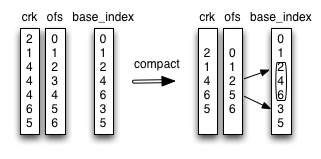
\includegraphics[]{images/d4_compaction_storage}
  \caption{Information about compactions are held in the offset array}
  \label{fig:compaction_causes_non_consecutive_offset_entries}
\end{figure}

The potential advantages of using compaction are that we can fit more edges into memory, that we can improve cache utilization by improving spatial locality among edge clusters within the edge array.

The costs for applying compaction are copying of memory upon compaction, traversing the AVL tree of the cracker index to update all the shifted entries upon compaction, and the maintenance of the  array of offsets.

\subsubsection{Algorithm Overview}

The format of the algorithm is almost the same as standard cracking. After a uniform column fragment is identified, that fragment is compacted. When returning a section of the column, if there are compacted values within the selection, they must be decompressed into the base index by using the offset array.

Figure \ref{fig:compaction_cracker_index_usage} compacting duplicated values results in changes within the cracker index to maintain correctness.

\begin{figure}[H]
  \centering
  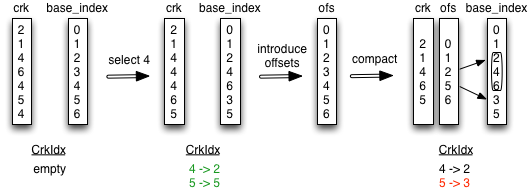
\includegraphics[width=\textwidth]{images/d5_compaction_cracker_index_usage}
  \caption{Compaction causes entries in the cracker index for greater values to be reduced}
  \label{fig:compaction_cracker_index_usage}
\end{figure}

The algorithm starts the same as for standard cracking, however, there is the added introduction of the offset column, which is initialized to 0, because before any compactions have been made, elements in the cracker column are not offset from elements in the base columns. The tightening phase is identical to that of standard cracking.

After the tightening phase, if a single value is identified as the only selected value, then we must check for compression by checking the cracker index to see if this value has been selected (and therefore compressed) before. If so then we can return immediately by decompressing the value at that index in the cracker column.

During the scan, previously compacted values in the cracker column are never swapped around. In our case it is impossible because a previously compressed column fragment will never be contained within a larger range query since our queries are for ranges of just a single node id. Even in the general case, swapping compacted values can be avoided by only cracking the boundary pieces - that is, by not scanning column fragments which are known to be included in the final result anyway, and instead physically reorganizing only the first and last fragments in the selected range.

Single values in the cracker column are swapped around just like for standard cracking, however, the $base\_index$ array may have a different length to the cracker column due to compactions, so the way swaps happen is changed slightly. We use the properties of the offset array to ensure that the correct swaps take place, under the knowledge that no compacted values will ever be swapped.

\begin{tcolorbox}
$\forall i: 0 \leq i < |crk|-1$, $\forall j: ofs[i] \leq j < ofs[i+1]$, $crk[i]$ = $base\_column[base\_index[j]]$
$\forall j: ofs[|crk|-1] \leq j < |base\_column|$, $crk[j]$ = $base\_column[base\_index[|crk|-1]]$
\end{tcolorbox}

With these properties in mind, we swap values in the base index found by passing the relevant pointers through the offset array first. That is, rather than swapping for example the elements at $L$ and $I$, instead we swap the values at $ofs[L]$ and $ofs[I]$.

Immediately after the scan the cracker index is updated and checked for compression opportunities. If the cracker index contains minimally different values, then the values of the smaller run can be compressed, because we know the index in the cracker column before which all entries are exceeded by that value, and also the index after which all values exceed that value. This is the principle of recognition compression, which is discussed in more detail in the next subsection. Figure \ref{fig:compaction_recognition} illustrates this.

\begin{figure}[H]
  \centering
  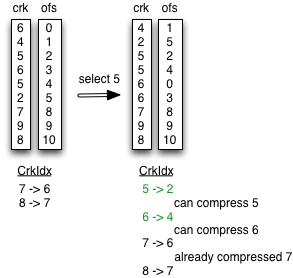
\includegraphics[]{images/d6_compaction_recognition}
  \caption{Minimally different values in the cracker index imply a compression opportunity}
  \label{fig:compaction_recognition}
\end{figure}

If a compression opportunity is found, the compaction is performed. This involves deleting the contiguous indices of the duplicated values for the cracker column and the offsets column. However, when we delete these values, the entries in the cracker column after the compacted value are shifted towards the head of the array. This means that their indices within the cracker column change, and therefore any entries in the cracker index to those values are incorrect. To amend this, all entries in the cracker index whose value is greater than the value being compacted have their index reduced by the number of values compacted. This is because entries in the cracker index with a greater value than the value being compacted necessarily appear later in the column and therefore are shifted during compaction. The reduction is by the number of values compacted, because this is the size of the shift and therefore the size of the required amendment to maintain correctness.

We must take care that the various potential compactions we can perform after the scan do not interfere with one another. Figure \ref{fig:compact_in_correct_order} indicates a scenario in which this can happen. In this diagram, a selection for the value 3 has just finished the scanning phase and is ready to go into compaction. By compacting the lower values first, the implementation must account for headward shifts in the cracker column's values, otherwise the insertion of the next value into the cracker index will be incorrect. In our solution, we address this problem by performing compactions in descending order of the value being compacted.

\begin{figure}[H]
  \centering
  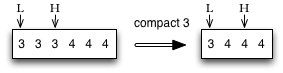
\includegraphics[]{images/d7_compaction_compact_in_correct_order}
  \caption{Compactions can affect each other, headward shifts in later sections of the array must be accounted for.}
  \label{fig:compact_in_correct_order}
\end{figure}

To protect against this problem, we can, as just mentioned, make sure to update pointers appropriately when doing multiple compactions in a single cracker select, or, as we have chosen to do in our implementation, do the compactions always from tail to head, such that there is no potential for interference. Two values are inserted into the cracker index after a selection. The value being selected, and the minimally greater value.

Finally, we return the results to the query. If any compactions took place, we follow the edge pointers from the cracking scan to the offset array and then into the base index, giving us the relevant indices of the base columns.

\subsection{Recognition}

After recognizing a section of column which can be compressed, we need it store this information somewhere in order to later exploit it.

If we are doing per-fragment compression, then we can recognize a compression opportunity when two values are stored in the cracker index which are minimally different. In this case, we need no extra storage - the cracker index contains all the information we need in order to be able to later exploit this.

Otherwise, if we are applying a run-length encoding across the column, we need a separate structure to hold the information about each of the runs, since the compressions are in this case applied at a finer level of granularity than the cracker index is fit to store information about.

The main advantage of recognition versus compaction is that it avoids the various performance costs associated with applying compaction. Additionally, we have found that recognition methods are easier to implement than compaction methods.

To demonstrate an example of how per-fragment recognition compression works, look back to figure \ref{fig:compaction_recognition}. In it, two uniform column fragments are shown at the end of a cracking scan, along with the two edge pointers and the current, unupdated cracker index. It is obvious that the selected column-fragment can be compressed, but the later column-fragment can now also be safely compressed for the same reason. We know in the cracker column the index before which all values are less and the index after which all values are greater, enabling us to exploit this uniform section in the future.

\section{Run-length encoding}

Our aim with run-length encoded (RLE) cracking is to be able to speed up the scan by enabling scanning pointers to hop over long runs of the same value. For this, we build and maintain information about all runs of consecutive nodes in the cracker column. This is done inside an array called $run\_lengths$. $run\_lengths[i]$ indicates to a scanning pointer that the next \texttt{i} values (inclusive) are the same, and therefore can be considered together, whether that means that they are hopped over, or swapped away to another part of the column. Crucially, this applies when encountering $run\_lengths[i]$ in either direction, however, the information about in which direction is not stored, it is assumed that a pointer always visits the "start" of the run in the direction it is traveling. This is an invariant of our implementation.

In compactive RLE, the bi-directionality of the run-lengths stored is trivial, because the duplicated values are all deleted anyway, and only materialize upon tuple reconstruction. However, the complications associated with compaction still apply.

For recognition RLE, the bi-directionality is not a given however, duplicated values are not compacted, meaning that the existence of a run must be marked on both ends, such that a forwards moving edge pointer arrives at the front-side of the run and a backwards moving edge pointer arrives at the tail-side of the run. Figure \ref{fig:rle_bidirectionality} illustrates why duplicating the run-length on both sides of the run is necessary.

\begin{figure}[H]
  \centering
  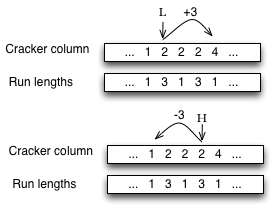
\includegraphics[]{images/d9_rle_bidirectionality}
  \caption{Both forwards and backwards moving pointers need knowledge about runs in order to exploit them}
  \label{fig:rle_bidirectionality}
\end{figure}

Note that the values of $run\_lengths$ within runs is not important, because in a correct implementation we will never read any of those values. In diagrams we will arbitrarily use 1s, although for our implementation any number in the range $[1, rl)$ can occur in $run\_lengths$ within a run of length $rl$.

We also need to maintain the $run\_lengths$ array under the restructuring that takes place during cracking to retain its consistency. We must ensure that the invariants associated with the edge pointers are maintained, and that the properties of $run\_lengths$ are preserved.

This must also take account of the fact that two runs of different length may need to be swapped during the scan. When making these swaps of different length runs, we may need to modify entries of $run\_lengths$ in order to correctly retain its properties. We have studied two approaches to swapping around runs of different lengths during the scanning phase.

The first approach to swapping two runs of different length is to swap the entire of the shorter run and modify entries of $run\_lengths$ corresponding to the longer run to maintain consistency after the swap. This means that the longer run is not fully swapped, so we have called it "underswapping". Underswapping causes the longer run to get broken up into two runs, one run the same size as the smaller run, which gets swapped entirely with the smaller run, and the other, a run consisting of the left-over section of the longer run, which is not swapped. Underswapping aims to be simple to implement while maintaining the scanning benefits of run-length encoding, however runs are often broken and so large gains are not made.

The basic concept is illustrated in figure \ref{fig:rle_underswapping}, in which the outlined green sections are swapped, the outlined red section stays still and the run length values outlined in blue have to be changed to preserve correctness of the $run\_lengths$ array after the swap.

\begin{figure}[H]
  \centering
  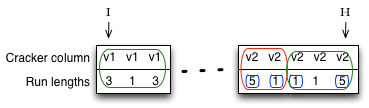
\includegraphics[]{images/d10_rle_underswapping}
  \caption{Example of Underswapping}
  \label{fig:rle_underswapping}
\end{figure}

The second approach is to swap the entire of the longer run, and pad the shorter run with more elements. This requires the padded elements to have their runs checked and potentially have entries modified, due to the possibility that they are constituents of another run. Due to the fact that the shorter run is swapped with more elements than are actually in that run (by padding), we call this "overswapping". Overswapping aims to preserve runs as much as possible, however it is also more complex. The diagram in figure \ref{fig:rle_overswapping} shows an example of using overswapping. The green outlined areas must be swapped, the red areas are also swapped with each other, and run lengths outlined in blue must be changed in order to retain run length correctness after the swap.

\begin{figure}[H]
  \centering
  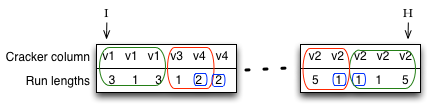
\includegraphics[]{images/d11_rle_overswapping}
  \caption{Example of Overswapping}
  \label{fig:rle_overswapping}
\end{figure}

Later in this section, we will discuss in detail the different cases for swapping around runs of different lengths, for both underswapping and overswapping. First we will look at the sections of algorithm that both of these RLE methods have in common.

\subsubsection{Algorithm Overview}

Both underswapping and overswapping implementations of cracking with RLE recognition compression share most of the algorithm in common. The only differences occur during the scan phase, however we will here describe the rest of the algorithm, which the two implementations share in common.

When the cracker column is initialized as a copy of the original column, $run\_lengths$ is also initialized. Its initial value is an array of the same length as the cracker column filled entirely with 1s.

The edge pointers are initialized from lookups into the cracker index and define the boundaries of the appropriate column-fragment, just like in other variants of the cracking algorithm.

The routines for tightening the pointers are different than for non-RLE variants, because the pointers move by the length of the run they are currently pointing to whenever they are tightened. Additionally, while tightening the edge pointers, we are looking for opportunities to build up and mark runs of duplicated values that they encounter.

When tightening the edge pointers in the tightening phase, we move pointers by jumping over each run, as well as building them up as we encounter them, while making sure to avoid under/overflow for cases where the value being sought isn't present. The way a run is built up during the tightening phase, using the low side pointer as an example, is shown in figure \ref{fig:rle_run_building}.

\begin{figure}[H]
  \centering
  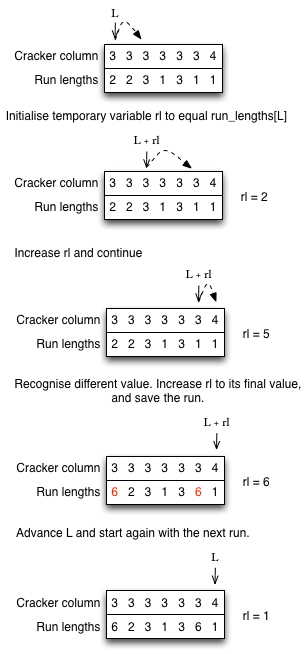
\includegraphics[]{images/d12_rle_run_building}
  \caption{Run building with the low edge pointer}
  \label{fig:rle_run_building}
\end{figure}

The case of swapping runs of different lengths between the low and iteration pointers is the same for both underswapping and overswapping, because we have the knowledge that the values at the indices in the range $[I, L)$ are all the value being queried for. This means that we can immediately make a run out of it and do as big a swap as possible, advancing the pointers as much as possible. We did experiment with using the strict underswapping and overswapping methods for these stages, however we found that the exploiting the information we knew about the intermediate values between $I$ and $L$ gave better performance than either of them. Later in this subsection we describe the low-side swaps in more detail.

When the iteration pointer is to be advanced during the scan, we can choose to try to build runs during the advancement, or not. After trialling both methods on our generated datasets, we found that trying to build runs causes the algorithm to slow down, so our final implementations don't do that.

Also during the scan, the tightening of pointers after making swaps is the same as for standard cracking, including the fact that if the low edge pointer overtakes the iteration pointer during tightening, the iteration pointer catches up immediately.

After the scan, we check that values were indeed selected - if the low edge pointer has surpassed the high edge pointer, then we know from their relative invariants that the sought value isn't present in the column. Figure \ref{fig:edge_pointers_pass_each_other} illustrates this fact.

\begin{figure}[H]
  \centering
  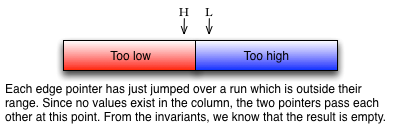
\includegraphics[]{images/d13_edge_pointers_pass_each_other}
  \caption{Two tessellating runs, neither of which are selected, form the boundary at which the edge pointers pass each other in a query returning no results.}
  \label{fig:edge_pointers_pass_each_other}
\end{figure}

Once the scan is finished, we combine into a single run the entire resultant fragment containing all instances of the value to be returned. We know this is the case for the same reason as when we do per-fragment compression. The insertion into the cracker index and returning of values is the same as for standard cracking.

\subsubsection{Low side swaps}

If the two runs to be swapped are the same length, then we can swap them immediately and entirely without doing anything else, because no runs are going to be invalidated and so none need to be edited.

If however they are different lengths, then we first change the situation in order to eliminate the possibility of having to deal with the situation in which values used to pad the shorter run spill into the longer run, creating an overlap. The change we make uses our knowledge that all the values of the cracker column lying within the index range $[L, I)$ are the selected value. We combine all of these values into a single run, resulting in the two runs to be swapped having a border just before the iteration pointer.

Our aim is to make the swap while preserving as much of the longer run as possible. To do this, we swap the entirety of the smaller run and edit the $run\_lengths$ array so that consistency is maintained.

\subsubsection{Low side swaps: Iteration run shorter}

Figure \ref{fig:rle_lowside_1a} shows the situation. The swap we intend to make is outlined in green and the run lengths to be amended are outlined in blue. We must ensure that after this swap takes place the properties of $run\_lengths$ are preserved.

\begin{figure}[H]
  \centering
  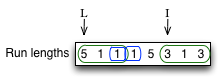
\includegraphics[]{images/d14_rle_lowside_1a}
  \caption{RLE low side swap, iteration run shorter: Swap recognized}
  \label{fig:rle_lowside_1a}
\end{figure}

Since we are swapping the full iteration pointer side run, we know that the last element getting swapped of those will be ending up at the tail end of our final run of selected values. Therefore we amend this entry in $run\_lengths$ with the number of values, which is equal to the difference between the two pointers, since all the values between them will constitute this run. Similarly, we know the element which will be at the start of the final run immediately follows the last element being swapped with the iteration run, so we amend that entry in $run\_lengths$ with the difference between the pointers as well. These amendments to $run\_lengths$ are shown in figure \ref{fig:rle_lowside_1b}.

\begin{figure}[H]
  \centering
  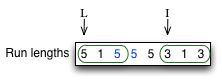
\includegraphics[]{images/d14_rle_lowside_1b}
  \caption{RLE low side swap, iteration run shorter: Run lengths entries amended}
  \label{fig:rle_lowside_1b}
\end{figure}

Having amended $run\_lengths$ appropriately, we can perform the full swap of the iteration side run with the appropriate number of elements from the low edge pointer, knowing that the resulting entries in the cracker column and $run\_lengths$ array will be consistent. Figure \ref{fig:rle_lowside_1c} shows the run lengths array after the swaps are completed.

\begin{figure}[H]
  \centering
  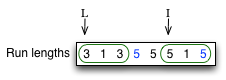
\includegraphics[]{images/d14_rle_lowside_1c}
  \caption{RLE low side swap, iteration run shorter: Swaps completed}
  \label{fig:rle_lowside_1c}
\end{figure}

At this point, we must advance the pointers to make progress in the scan. We know that the run we just swapped down to the low edge pointer contains values less than the selected node id, so the low edge pointer should be advanced beyond them. Also, the iteration pointer is now in the middle of a run, which is dangerous, so we get it out of there by advancing it to the end of that run. We don't swap it to the beginning because we know that it is a run containing the node id under selection - no need to scan it. The diagram in figure \ref{fig:rle_lowside_1d} demonstrates the advancing of the pointers.

\begin{figure}[H]
  \centering
  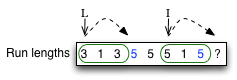
\includegraphics[]{images/d14_rle_lowside_1d}
  \caption{RLE low side swap, iteration run shorter: Pointers tightened}
  \label{fig:rle_lowside_1d}
\end{figure}

\subsubsection{Low side swaps: Iteration run longer}

In this situation, the shorter low-side run must be swapped to the end of the iteration run. We must again edit $run\_lengths$ to maintain consistency, as we can be seen from figure \ref{fig:rle_lowside_2a}.

\begin{figure}[H]
  \centering
  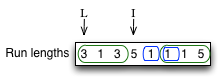
\includegraphics[]{images/d15_rle_lowside_2a}
  \caption{RLE low side swap, iteration run shorter: Swap recognized}
  \label{fig:rle_lowside_2a}
\end{figure}

The first element of the iteration run swapped with the low-side run must have its run-length changed, as well as the last element of the iteration run that is not swapped, so that after the swap, both sides of the run are still marked. The arithmetic for finding these positions is straightforward. Figure \ref{fig:rle_lowside_2b} shows the same situation as above but with the necessary amendments.

\begin{figure}[H]
  \centering
  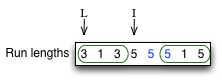
\includegraphics[]{images/d15_rle_lowside_2b}
  \caption{RLE low side swap, iteration run longer: Run lengths entries amended}
  \label{fig:rle_lowside_2b}
\end{figure}

After the amendments, the entire low-side run is swapped to the end of the iteration run, and the updated run markings mean that the iteration run is again wholly preserved, which you can see in the figure \ref{fig:rle_lowside_2c} .

\begin{figure}[H]
  \centering
  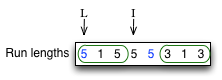
\includegraphics[]{images/d15_rle_lowside_2c}
  \caption{RLE low side swap, iteration run longer: Swaps completed}
  \label{fig:rle_lowside_2c}
\end{figure}

Finally, the pointers must be updated. The low pointer can hop over the swapped back run, since we know that its duplicated value is less than the selected value. The iteration pointer moves to the start of the run that was swapped forwards, the position of which was calculated earlier. Figure \ref{fig:rle_lowside_2d} shows how the pointers are updated.

\begin{figure}[H]
  \centering
  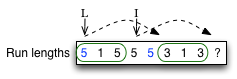
\includegraphics[]{images/d15_rle_lowside_2d}
  \caption{RLE low side swap, iteration run longer: Pointers advanced}
  \label{fig:rle_lowside_2d}
\end{figure}

\subsection{Underswapping Scan}

Underswapping is the simpler of the two approaches, because it has fewer edge cases to consider. We have only to amend the two pieces of the broken longer run before swapping all the values from the smaller run across to the equally sized run just created from a piece of the longer run. This method wastes some information we have acquired, but is fairly simple.

Within the cracking scan, if the run at the iteration pointer is to be swapped, it will either be swapped with the run at the low edge pointer or the high edge pointer. If the runs have equal length, they can be swapped immediately with no further amendments. Otherwise, the run which is longer can either be the run getting swapped towards the middle or towards the edge.

Under the following headers, we describe and illustrate the algorithm's behavior given the circumstance of the run at the iteration pointer. The two cases are all fairly similar and straightforward. We have lay them out in series of diagrams, starting at the initial situation, and ending with the runs swapped and the pointers appropriately tightened for the next iteration.

\subsubsection{High side swaps: Iteration run shorter}

The diagram in figure \ref{fig:underswapping_1a} shows the situation once we have identified that we are doing a high-side swap and the iteration run is shorter. The sections to be swapped are outlined in green and the run lengths which need to be amended are outlined in blue. We do not know about the intermediate values between the two runs, if there are any, so we have included an ellipsis in the depiction of the column to indicate these values.

\begin{figure}[H]
  \centering
  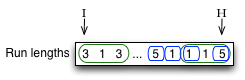
\includegraphics[]{images/d18_underswapping_1a}
  \caption{Underswapping high side run, iteration run shorter: Swap recognized}
  \label{fig:underswapping_1a}
\end{figure}

Figure \ref{fig:underswapping_1b} shows the amendments, which are shown with blue font. Due to underswapping, we can see that the long run of 5 has been broken into a run of 2 and a run of 3 in order to facilitate the swap. Below the run lengths array in the diagram is the cracker column, which we have filled with two generic values - $i$ for the duplicated value in the iteration run, and $h$, the duplicated value in the high-side run.

\begin{figure}[H]
  \centering
  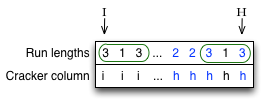
\includegraphics[]{images/d18_underswapping_1b}
  \caption{Underswapping high side run, iteration run shorter: Run lengths entries amended}
  \label{fig:underswapping_1b}
\end{figure}

After the swap, the values are moved and the correctness of run lengths and the cracker column is maintained from the amendments. We can also see that the run of $i$, known to be too great to be included in the selection, has been moved to the high-pointer and is ready to be hopped over.

\begin{figure}[H]
  \centering
  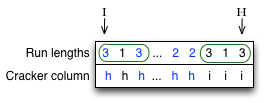
\includegraphics[]{images/d18_underswapping_1c}
  \caption{Underswapping high side run, iteration run shorter: Swaps completed}
  \label{fig:underswapping_1c}
\end{figure}

Finally, in figure \ref{fig:underswapping_1d} we show the tightening of the high pointer in which it hops over the swapped-up run.

\begin{figure}[H]
  \centering
  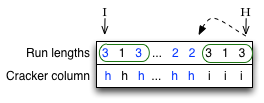
\includegraphics[]{images/d18_underswapping_1d}
  \caption{Underswapping high side run, iteration run shorter: High pointer tightened}
  \label{fig:underswapping_1d}
\end{figure}

\subsubsection{High side swaps: Iteration run longer}

As before, the sections to be swapped are outlined in green and the run lengths which need to be amended are outlined in blue. The ellipsis is also used in the same way as it was under the previous header. The situation is shown in figure \ref{fig:underswapping_2a}.

\begin{figure}[H]
  \centering
  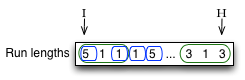
\includegraphics[]{images/d19_underswapping_2a}
  \caption{Underswapping high side run, iteration run longer: Swap recognized}
  \label{fig:underswapping_2a}
\end{figure}

Figure \ref{fig:underswapping_2b} shows the arrays after amending the necessary run lengths.

\begin{figure}[H]
  \centering
  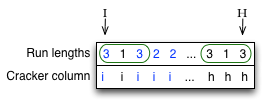
\includegraphics[]{images/d19_underswapping_2b}
  \caption{Underswapping high side run, iteration run longer: Run lengths amended}
  \label{fig:underswapping_2b}
\end{figure}

The amendments mean that after the swaps the runs are still all correct, as shown in figure \ref{fig:underswapping_2c}.

\begin{figure}[H]
  \centering
  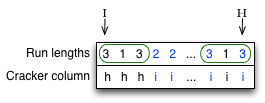
\includegraphics[]{images/d19_underswapping_2c}
  \caption{Underswapping high side run, iteration run longer: Swaps completed}
  \label{fig:underswapping_2c}
\end{figure}

Finally, the high edge pointer hops over the swapped up run to tighten the region to scan. This is shown in the diagram in figure \ref{fig:underswapping_2d}.

\begin{figure}[H]
  \centering
  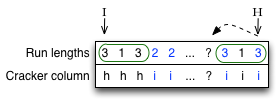
\includegraphics[]{images/d19_underswapping_2d}
  \caption{Underswapping high side run, iteration run longer: High pointer tightened}
  \label{fig:underswapping_2d}
\end{figure}

\subsection{Overswapping Scan}

When overswapping, we swap the entire of the longer run, and pad the shorter run to length. The runs within the padding must be amended to remain consistent, and if the padding contains partial runs, then those runs must be amended outside the padding as well to remain consistent after the swap. Additionally, if the padding causes the two swapped regions to overlap, then we don't have to swap all of the values - a saving that requires us to also make updates into $run\_lengths$ to preserve correctness.

Unlike in the low-side swap case, we know nothing about the values between the iteration pointer and high pointer, other than that the value at the high pointer is not greater than \textit{x}.

\subsubsection{High side swaps}

As with low side swaps, when the runs are the same length, we can immediately swap them without any fuss and advance the edge pointer appropriately.

For high side swaps of unequal length, we have no information about the intermediate values between the two runs being swapped, therefore we have to manage the padding and ensure that no inconsistencies are introduced into $run\_lengths$ as a result. This includes the possibility that the padding may spill into the longer run and the possibility that the padding may form part of another separate run, causing that run to potentially become broken apart. We describe the first of these possibilities as "overlapping" because the padded shorter run overlaps with the longer run. The second we describe as the padding having a remainder, requiring amendments to $run\_lengths$.

In our description of high-side overswapping, we will first describe the case in which the padding overlaps with the longer run. Then to describe non-overlapping padding, we will describe the strategy we used to deal with padding which has a remainder, followed by an explanation of the swaps which take place after the padding has been prepared.

\subsubsection{Overlapping}

Figure \ref{fig:overswapping_overlapping} is an illustration of the two possible cases of overlapping when swapping high-side runs. The values in the longer run which are also part of the padding are shown in red font.

\begin{figure}[H]
  \centering
  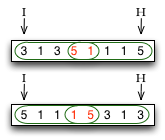
\includegraphics[]{images/d20_overswapping_overlapping}
  \caption{Padding can overlap with the longer run.}
  \label{fig:overswapping_overlapping}
\end{figure}

This problem is just like the low-side swap cases, but with slightly different arithmetic because $H$ points to the tail end of its run. Because we assume that the $run\_lengths$ array is consistent, we know that we can take padding right up to the border with the other run and know that there is no possibility that the padding has any remainder. From this position we swap all the values between the iteration and high pointers except for the overlapping region, after making some adjustments in the longer run.

After the amendments are made we swap the two sections, the longer run aligns so consistency is preserved and the longer run is fully preserved.

\subsubsection{Padding Remainder}

The problem here is that the padding may contain for example two out of three elements of a run, meaning that if the padding gets swapped, the run will be broken. The padding may contain multiple runs - we need only check the last one. The ideal case is for the last run in the padding to be entirely contained within it, that is, the padding has no remainder.

Our approach to fixing padding remainder is to use underswapping. We break the padded run into a run inside the padding and a run outside the padding.

The implementation of this method is that we first initialize a padding pointer, with a view to move it through the padding until finding the last run. We then check if the padding has a remainder or not. If it doesn't, we don't need to do anything, otherwise, we fix the remainder into two runs as described in the previous paragraph.

Although the padding extends in different directions depending on which side it's on, the only thing that changes is the necessary arithmetic to fix the remainder if there is one, and to calculate the location of the swaps. We illustrate in figure \ref{fig:padding_remainder} the amendments that must be made due to the padding remainder both in the case where the iteration run is longer and in the case where the high run is longer. 

\begin{figure}[H]
  \centering
  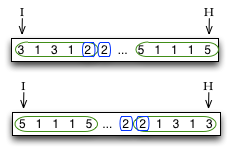
\includegraphics[]{images/d22_padding_remainder}
  \caption{Padding can contain partial runs which must be amended.}
  \label{fig:padding_remainder}
\end{figure}

\subsubsection{Padding Swaps}

At the stage at which we start to consider doing swaps, we have two equal length sections of column. The longer run is one of these sections, it is uniform. The other contains a run whose value we know and want to swap to the far side of the longer run, plus some padding to bring it up to length. The padding contains only whole runs and no runs will be broken by swapping it away, either by coincidence or because we have explicitly amended it.

We consider both of the two sections in two different parts. The shorter run, and the part of the longer run which will be swapped with it, are both one part, which we call the main part, because it constitutes the reason why we are doing the swap in the first place. The padding of the shorter run, and the corresponding part of the longer run we call the padding part, or just "the padding". In both the case where the iteration run is longer and where it is shorter, the padding is towards the middle-ground between the iteration and high pointers, as you can see from figure \ref{fig:padding_remainder}. After the swap therefore, the relative order of the main and padding parts will be swapped, meaning that we will have to make amendments in the longer run in order to preserve it. The run length entries which must be amended are outlined in blue in figure \ref{fig:padding_swaps_amendments}.

\begin{figure}[H]
  \centering
  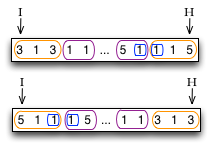
\includegraphics[]{images/d23_padding_swaps_amendments}
  \caption{Amendments in the runs for swapping both the main and padding parts during a high-side overswap.}
  \label{fig:padding_swaps_amendments}
\end{figure}

After the swap we are left with the iteration run swapped up and the $run\_lengths$ array in a correct state. Finally we tighten the high pointer by hopping it over the run that got swapped up. This is illustrated in figure \ref{fig:padding_swaps_done}.

\begin{figure}[H]
  \centering
  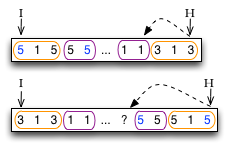
\includegraphics[]{images/d25_padding_swaps_done}
  \caption{Tightening the high pointer after a completed high-side overswap.}
  \label{fig:padding_swaps_done}
\end{figure}